% !TeX root = ../main.tex
\chapter{実験}
\label{chap:experiment}

\section{実験の条件}
\label{sec:condition}
% 表の参照は Table~\ref{tab:...}
これは記入例のためのダミーの文である．
実験の条件をTable~\ref{tab:condition}に示す．

% 表：キャプションは表の上に置く．配置の指定は [b]
% 単位付きの数値は \SI{数値}{単位}
\begin{table}[b]
  \centering
  \caption{実験の条件}
  \label{tab:condition}
  \begin{tabular}{lr}
    \toprule
    項目 & 値 \\
    \midrule
    試行回数 & 10 \\
    計測距離 & \SI{1.5}{m} \\
    サンプリング周期 & \SI{100}{ms} \\
    \bottomrule
  \end{tabular}
\end{table}

\section{実験の結果}
\label{sec:result}
これは記入例のためのダミーの文である．
試行回数と誤差の関係をFig.~\ref{fig:result}に示す．

% キャプションに \cite や \ref を書くときは，[] に図目次用の短い文を書く
\begin{figure}[t]
  \centering
  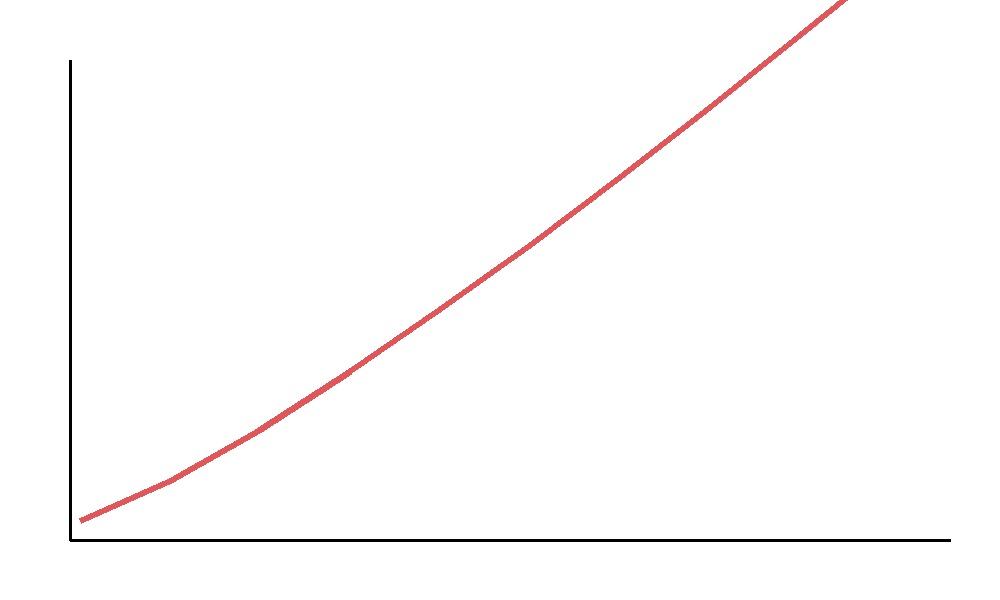
\includegraphics[width=0.7\linewidth]{fig/result.png}
  \caption[試行回数と誤差の関係]{試行回数と誤差の関係（文献\cite{example2025}と同じ条件）}
  \label{fig:result}
\end{figure}
